\documentclass[12pt,border=12pt]{standalone}
\usepackage[utf8]{inputenc}
\usepackage[utf8]{vietnam}

\usepackage{amsmath}
\usepackage{amsfonts}
\usepackage{amssymb}

\usepackage{tikz}
\usetikzlibrary{arrows, decorations.markings, calc, fadings, decorations.pathreplacing, patterns, decorations.pathmorphing, positioning}
\tikzset{middlearrow/.style={
    decoration={markings,
    mark= at position 0.5 with {\arrow{#1}},
    },
    postaction={decorate}
    }
}


\begin{document}
    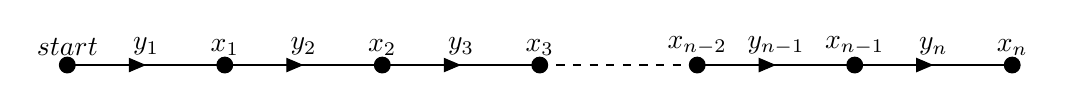
\begin{tikzpicture}[>=triangle 45]
        \draw[fill = black] (0, 0) circle (0.1) node[above] {$start$} ;
        \draw[middlearrow={>}] (0, 0) -- (2, 0);
        \draw (1, 0) node[above] {$y_1$};
        \draw[fill = black] (2, 0) circle (0.1) node[above] {$x_1$};
														
        \draw[middlearrow={>}] (2, 0) -- (4, 0);
        \draw (3, 0) node[above] {$y_2$};
        \draw[fill = black] (4, 0) circle (0.1) node[above] {$x_2$};
					
        \draw[middlearrow={>}] (4, 0) -- (6, 0);
        \draw (5, 0) node[above] {$y_3$};
        \draw[fill = black] (6, 0) circle (0.1) node[above] {$x_3$};
					
        \draw[dashed] (6, 0) -- (8, 0);
        \draw[fill = black] (8, 0) circle (0.1) node[above] {$x_{n-2}$};
					
        \draw[middlearrow={>}] (8, 0) -- (10, 0);
        \draw (9, 0) node[above] {$y_{n-1}$};
        \draw[fill = black] (10, 0) circle (0.1) node[above] {$x_{n-1}$};
					
        \draw[middlearrow={>}] (10, 0) -- (12, 0);
        \draw (11, 0) node[above] {$y_n$};
        \draw[fill = black] (12, 0) circle (0.1) node[above] {$x_n$};
    \end{tikzpicture}
\end{document}